\documentclass{beamer}

\usepackage{beamerthemesplit}
\usetheme{Singapore} %Copenhagen}
%\usecolortheme{whale}

%\usepackage[T2A]{fontenc}
%\usepackage[utf8]{inputenc}
%\usepackage[russian]{babel}

\usepackage[main=russian,english]{babel}   %% загружает пакет многоязыковой вёрстки
\usepackage{fontspec}      %% подготавливает загрузку шрифтов Open Type, True Type и др.
\defaultfontfeatures{Ligatures={TeX},Renderer=Basic}  %% свойства шрифтов по умолчанию
\setmainfont{Times New Roman} %% задаёт основной шрифт документа
%\usefonttheme{professionalfonts}% SOLUTION
\usefonttheme{serif}

\usepackage{hyperref}
\usepackage{textcomp}
\usepackage{amssymb,amsmath}
%\usepackage{animate}
%\usepackage{longtable}
\usepackage{xcolor}

%\usepackage{pgffor}
\usepackage{enumitem}
\usepackage[export]{adjustbox}

\newcounter{N}

%% Форматирование окружения itemize
%\usepackage{ragged2e}
%\let\olditem\item
%\renewcommand\item{\olditem\justifying}

\usepackage{ mathrsfs }
\newcommand{\Rho}{\mathscr{P}}

\renewcommand{\Re}{\operatorname{Re}}

\newcommand{\argxi}{(\xi^1,\xi^2,\xi^3)}
\newcommand{\argx}{(x^1,x^2,x^3)}

\newcommand{\argxiv}{(\vec{\xi})}
\newcommand{\argxv}{(\vec{x})}


\newcommand{\argxbarn}{(\bar{x}^1,\bar{x}^2,\ldots, \bar{x}^n)}
\newcommand{\argxn}{(x^1, x^2,\ldots, x^n)}

\newcommand{\argtxi}{(t, \xi^1,\xi^2,\xi^3)}
\newcommand{\argtoxi}{(t_0, \xi^1,\xi^2,\xi^3)}

\newcommand{\argtxiv}{(t, \vec{\xi})}
\newcommand{\argtoxiv}{(t_0, \vec{\xi})}


\newcommand{\argtx}{(t, x^1,x^2,x^3)}
\newcommand{\argtox}{(t_0, x^1,x^2,x^3)}

\newcommand{\argtxv}{(t, \vec{x})}
\newcommand{\argtoxv}{(t_0, \vec{x})}


\newcommand{\pd}[2]{\frac{\partial #1}{\partial #2}}
\newcommand{\pdk}[2]{\frac{\partial^2 #1}{\partial #2^2}}

\newcommand{\od}[2]{\frac{d #1}{d #2}}
\newcommand{\odk}[3]{\frac{d^{#3} #1}{d #2^{#3}}}

\newcommand{\grad}{\operatorname{grad}}
\newcommand{\rot}{\operatorname{rot}}
\newcommand{\divo}{\operatorname{div}}

\title[]{Трёхмерные осесимметричные потенциальные течения идеальной жидкости}

\author[]{ {\em Верещагин Антон Сергеевич}
\\
канд. физ.-мат. наук, старший преподаватель\\
\bigskip
Кафедра аэрофизики и газовой динамики ФФ НГУ}

\usebackgroundtemplate{
\includegraphics[width=\paperwidth]{../img/background.png}}

\begin{document}
	
\frame{\titlepage}


\frame{
	\frametitle{Аннотация}
	\parbox{\textwidth}{
		Трехмерные потенциалы при течении идеальной жидкости. Потенциалы простейших течений. Обтекание сферы, парадокс Даламбера. Функция тока в осесимметричном случае. Связь между функцией тока и потенциалом. Обтекание тел вращения.
	}
}

\frame{
	\frametitle{ Основные определения}
	
	\begin{exampleblock}{Определение}
	\parbox{\textwidth}{
		Течение называется \alert{осесимметричным}, если существует такая прямая $l$, что во всех плоскостях, проходящих через $l$ картина течения одинакова и траектория жидкой частицы лежит в полуплоскостях, проходящих через $l$.
		
	}
	\end{exampleblock}

	\begin{exampleblock}{Определение}
		\parbox{\textwidth}{
			Течение называется \alert{потенциальным}, если в некоторой области пространства можно определить потенциал $\varphi(t,x,y,z)$, такой что
			\[
			\vec{v} = \grad \varphi.
			\]
			
		}
	\end{exampleblock}

}



\frame{
	\frametitle{Основные уравнения}
	
	\parbox{\textwidth}{
	Для трёхмерных потенциальных течений идеальной жидкости определённых в некоторой области пространства справедливы следующие уравнения.	
	}
	
	\bigskip
	
	
	\begin{exampleblock}{Уравнение неразрывности}
		\parbox{\textwidth}{
			\[
				\divo\vec{v}=\Delta\varphi = 0,\quad
				\vec{v}=\nabla \varphi
			\]
		}
	\end{exampleblock}
	
	\begin{exampleblock}{Интеграл Коши}
		\parbox{\textwidth}{
			\[
			\frac{\nabla\varphi^2}{2} + \frac{p}{\rho} = f(t)\footnote{Считаем, что поле внешних сил отстутствует}
			\]
			
		Интеграл Коши позволяет найти распределение давления по заданному потенциалу, определённому из уравнения неразрывности ($\rho=const$).
		}
	\end{exampleblock}
}

\frame{
	\frametitle{ Уравнение неразрывности в различных системах координат}
	
	\begin{exampleblock}{Сферическая система координат $r$, $\theta$, $\lambda$}
		\parbox{\textwidth}{
			\[
			\frac{1}{r^2 \sin\theta}
			\left\{
			\pd{}{r}\left( r^2 \sin\theta \pd{\varphi}{r} \right) + 
			\pd{}{\theta} \left( \sin\theta \pd{\varphi}{\theta} \right) +
			\pd{}{\lambda}\left( \frac{1}{\sin\theta} \pd{\varphi}{\lambda} \right)
			\right\}
			 = 0,
			\]
			где
			\[
			v_r = \pd{\varphi}{r},\quad
			v_\theta = \frac{1}{r}\pd{\varphi}{\theta},\quad
			v_\lambda = \frac{1}{r\sin\theta} \pd{\varphi}{\lambda}.
			\]
		}
	\end{exampleblock}
	
	
		\begin{columns}
		\begin{column}{0.7\textwidth}
			\parbox{\textwidth}{
				В случае осесимметричного течения можно пренебречь зависимостью $\varphi$ от $\lambda$.
			}
		\end{column}
	
		\begin{column}{0.3\textwidth}
			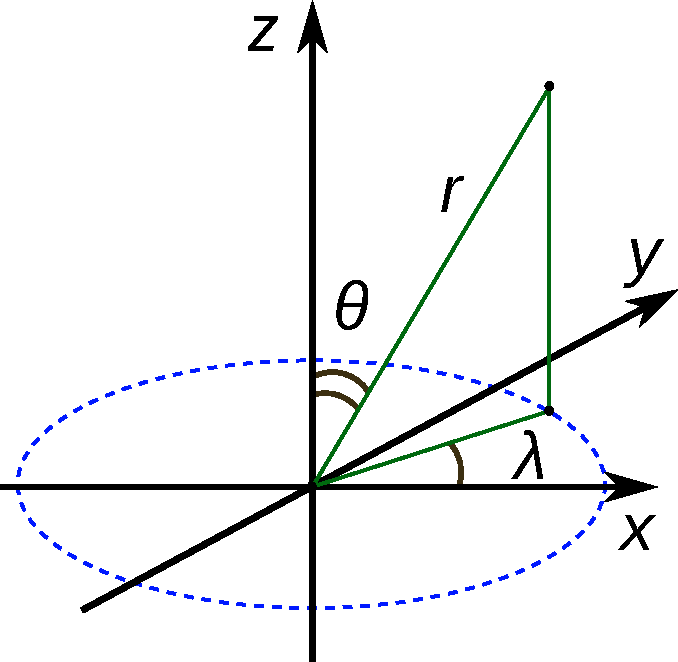
\includegraphics[width=\linewidth]{../img/sphere_origin.pdf}			
		\end{column}
	
	\end{columns}

}

\frame{
	\frametitle{ Уравнение неразрывности в различных системах координат}
	
	\begin{exampleblock}{Цилиндрическая система координат $r$, $\theta$, $z$}
		\parbox{\textwidth}{
			\[
			\frac{1}{r}
			\left\{
			\pd{}{r}\left( r v_r \right) + 
			\pd{}{\theta} v_\theta +
			\pd{}{\lambda}\left( r v_z \right)
			\right\}
			= 0,
			\]
			где
			\[
			v_r = \pd{\varphi}{r},\quad
			v_\theta = \frac{1}{r}\pd{\varphi}{\theta},\quad
			v_z =  \pd{\varphi}{z}.
			\]
		}
	\end{exampleblock}
	

	\parbox{\textwidth}{
		В случае осесимметричного течения вдоль оси $Oz$ можно пренебречь зависимостью $\varphi$ от $\theta$.
	}


}

\frame{
	\frametitle{ Источник в пространстве}
	
	\begin{exampleblock}{Сферически симметричное течение}
		\parbox{\textwidth}{
			\[
			\varphi = \varphi(r) \quad \Rightarrow \quad
			\pd{}{r}\left( r^2 \od{\varphi}{r} \right) = 0.
			\]
			
		}
	\end{exampleblock}\pause
	
	\begin{exampleblock}{Потенциал источника, расположенного в точке с координатами $(a,b,c)$}
		\parbox{\textwidth}{
			\[
				\varphi(x,y,z) = -\frac{q}{4\pi \sqrt{(x-a)^2+(y-b)^2+(z-c)^2}}.
			\]
			
		}
	\end{exampleblock}\pause
	
	\begin{exampleblock}{Расход жидкости через любую поверхность, охватывающую центр источника S}
		\parbox{\textwidth}{
			\[
			q = \int\limits_S v_n dS = \int\limits_S \pd{\varphi}{n} dS.
			\]
			
		}
	\end{exampleblock}
}

\frame{
	\frametitle{Диполь в пространстве}
	
	\begin{exampleblock}{Потенциал}
		\parbox{\textwidth}{
			Рассмотрим источник и сток одной и той же обильности $q$, находящиеся на оси $Oz$ на расстоянии $l$ друг от друга. Тогда их суммарный потенциал будет иметь вид
			\[
			\varphi =  -\frac{q}{4\pi \sqrt{x^2+y^2+(z-l/2)^2}} +
						\frac{q}{4\pi \sqrt{x^2+y^2+(z+l/2)^2}}.
			\]\pause
			
			При переходе к пределу при $l \to 0 $, а $q \to \infty$, причём $ql = M$, получится предельный потенциал
			\[
			\varphi = -\frac{Mz}{4\pi r^3} \quad \text{или} \quad
			\varphi = -\frac{M}{4\pi} \pd{}{l}\left(\frac{1}{r}\right),
			\]
			где $M$ -- момент диполя; $l$ -- направление оси диполя.
		}
	\end{exampleblock}
	
}

\frame{
	\frametitle{ Обтекание сферы }
	
	\begin{exampleblock}{Постановка}
		\parbox{\textwidth}{
			Требуется найти распределение скорости и давления при потенциальном обтекании сферы радиуса $R$, движущейся поступательно вдоль оси $Oz$ со скоростью $u$, в потоке идеальной жидкости, имеющей на бесконечности скорость $V$, направленную вдоль оси $Oz$, и давление $p_\infty$.
		}
	\end{exampleblock}
	
	\centering
	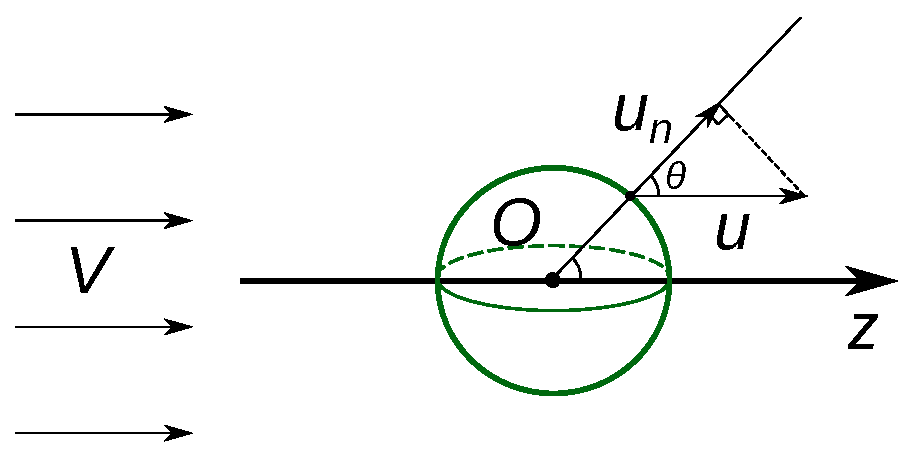
\includegraphics[width=0.7\textwidth]{../img/sphere.pdf}
	

	
	
}

\frame{
	\frametitle{ Математическая постановка }
		\begin{exampleblock}{Основные уравнения}
		\parbox{\textwidth}{
			В сферической системе координат пренебрегаем зависимостью от $\lambda$. Тогда для функции $\varphi = \varphi(r,\theta)$ запишем уравнение неразрывности
			\[
			\pd{}{r}\left( r^2 \sin\theta \pd{\varphi}{r} \right) +
			\pd{}{\theta} \left( \sin\theta\pd{\varphi}{\theta} \right) = 0.
			\]
		}
	\end{exampleblock}
	
	\begin{exampleblock}{Граничные условия на сфере}
		\parbox{\textwidth}{
			\[
			v_n = \left. \pd{\varphi}{n} \right|_{r=R} = u \cos\theta.
			\]
		}
	\end{exampleblock}

	\begin{exampleblock}{Граничные условия на бесконечности}
		\parbox{\textwidth}{
			\[
			v_r = \left. \pd{\varphi}{r} \right|_{r\to\infty} = V \cos\theta,\quad
			v_\theta = \frac{1}{r} \left. \pd{\varphi}{\theta} \right|_{r\to\infty} = -V \sin\theta.
			\]
		}
	\end{exampleblock}
}

\frame{
	\frametitle{ Решение задачи об обтекании сферы }
	
	\begin{exampleblock}{Упрощение}
		\parbox{\textwidth}{
			Пусть $\varphi(r,\theta) = Q(r) \cos\theta$, тогда уравнение неразрывности будет иметь вид
			\[
			r^2 \odk{Q}{r}{2} + 2r\od{Q}{r} - 2Q = 0.
			\]
		}
	\end{exampleblock}

	\begin{exampleblock}{Аналитическое решение}
		\parbox{\textwidth}{
			\[
			\varphi(r,\theta) = \left(Vr + \frac{V-u}{2} \frac{R^3}{r^2}\right) \cos\theta,
			\]
			которое можно переписать в виде
			\[
			\varphi = Vz- \frac{R^3}{2}(V-u) \pd{}{z}\left( \frac{1}{r} \right).
			\]
			
			Видно, это сумма потенциала поступательного движения потока со скоростью $V$ и потенциала диполя с моментом  $M = 2\pi R^3 (u-V)$.
		}
	\end{exampleblock}

	
}

\frame{
	\frametitle{ Обтекание покоящейся сферы }
	
	\parbox{\textwidth}{
	Если $u=0$, тогда
	\[
	\varphi = V \left(r+\frac{1}{2}\frac{R^3}{r^2}\right) \cos\theta
	\]
	и
	\[
		v_r = V \left(1 - \frac{R^3}{r^3}\right) \cos\theta,\quad
		v_\theta = -V \left(1 + \frac{R^3}{2r^3}\right) \sin\theta.
	\]

	Максимальное значение скорости на поверхности сферы достигается в точках $\theta=\pm\pi/2$ и равно $3/2V$.

	}


	
}

\frame{
	\frametitle{ Парадокс Даламбера для покоящейся сферы}
	
	\begin{exampleblock}{Интеграл Бернулли}
		\parbox{\textwidth}{
			Так как течение потенциально и стационарно, то 
			\[
			\frac{v^2}{2} + \frac{p}{\rho} = \frac{V^2}{2} + \frac{p_\infty}{\rho}
			\]
			
		}
	\end{exampleblock}
	
	\begin{exampleblock}{Выражение для давления}
		\parbox{\textwidth}{
			\[
			\frac{p-p_\infty}{\rho} = \frac{V^2}{2}\left( 1- \frac{9}{4} \sin^2 \theta \right)
			\]
			
		}
	\end{exampleblock}

	\parbox{\textwidth}{
	Суммарная сила, вызванная давлением потенциального течения жидкости на покоящуюся сферу, равна 0, вследствие симметрии распределения сил давления. Это называется \alert{парадоксом Даламбера}.
	}
	
	
}

\frame{
	\frametitle{ Функция тока для осесимметричных течений }
	
	\begin{exampleblock}{Уравнение неразрывности в цилиндрической системе координат с осевой симметрией в переменных $(r,z)$}
		\parbox{\textwidth}{
		\[
			\divo \vec{v} = \pd{}{r}(r v_r) + \pd{}{z}(r v_z) = 0\quad \Rightarrow \quad
			\pd{}{r}(r v_r)  = -\pd{}{z}(r v_z).
		\]	
		}
	\end{exampleblock}
	\begin{exampleblock}{Существование полного дифференциала}
		\parbox{\textwidth}{
			\[
			d\psi = r v_r dz - r v_z dr = \pd{\psi}{z} dz + \pd{\psi}{r} dr
			\]
			является полным дифференциалом (см. теорию про интегрирующий множитель).
		}
	\end{exampleblock}
	\begin{exampleblock}{Определение}
		\parbox{\textwidth}{
		Функцию $\psi(r,z)$  такую, что
		$
		v_r = \displaystyle\frac{1}{r}\pd{\psi}{z}$,
		$v_z = -\displaystyle\frac{1}{r}\pd{\psi}{r}
		$
		называют \alert{функцией тока для осесимметричных течений}.	
		}
	\end{exampleblock}
}

\frame{
	\frametitle{Свойства функции тока }
	
	\begin{exampleblock}{Постоянство на линиях тока}
		\parbox{\textwidth}{
			Уравнения линий тока в случае осесимметричного течения
			\[
			\frac{dr}{v_r} = \frac{dz}{v_z},
			\]
			поэтому на линиях тока 
			\[
			v_r dz - v_z dr = 0,
			\]
			следовательно
			\[
			d\psi = r (v_r dz - v_z dr) = 0
			\]
			и $\psi = const$.

			
		}
	\end{exampleblock}
	
}

\frame{
	\frametitle{ Свойства функции тока }
	
	\begin{columns}
		\begin{column}{0.35\textwidth}
			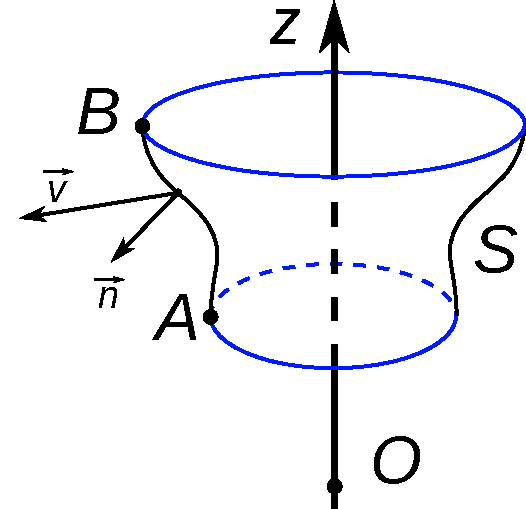
\includegraphics[width=\textwidth]{../img/streamfunction_flow.pdf}
		\end{column}
		\begin{column}{0.65\textwidth}

\begin{exampleblock}{Поток жидкости через поверхность $S$}
	\parbox{\textwidth}{
					
		\[
		\int\limits_S \vec{v}\cdot\vec{n} ds = 
		\int\limits_{0}^{2\pi}  \int\limits_B^A \left( v_z n_z + v_r n_r \right) r d\theta dl = 
		\]
		\[
		=
		2 \pi \int\limits_0^{l_0} \left( \left(-\frac{1}{r}\pd{\psi}{r} \right) \left(-\pd{r}{l}\right) + \frac{1}{r}\pd{\psi}{z} \pd{z}{l} \right) r dl=
		\]
		\[
		=
		2\pi\int\limits_0^{s_0} \od{}{l} \psi(r(l),z(l)) dl = 2\pi(\psi(A) - \psi(B)),
		\]
		\[
		r=r(l),\quad z=z(l),
		\]
		\[
		(r,z)|_{l=0} = B,\quad
		(r,z)|_{l=l_0} = A.
		\]
		
	}
\end{exampleblock}			
		\end{column}
	\end{columns}
}
\frame{
	\frametitle{ Связь функции тока и потенциала для осесимметричных течений}
	
	\begin{exampleblock}{Соотношения}
		\parbox{\textwidth}{
			\[
				\pd{\varphi}{r} = \frac{1}{r}\pd{\psi}{z},\quad
				\pd{\varphi}{z} = -\frac{1}{r}\pd{\psi}{r}
			\]
			Полученные соотношения \alert{отличаются} от условий Коши-Римана.
		}
	\end{exampleblock}\pause

	\begin{exampleblock}{Уравнение для функции тока}
		\parbox{\textwidth}{
			\[
			\pdk{\psi}{r}+\pdk{\psi}{z} \alert{-} \frac{1}{r}\pd{\psi}{r} = 0
			\]
			
			Полученное соотношение не является уравнением Лапласа, записанным в цилиндрической системе координат. В случае осесимметричных течений не работают методы ТФКП. В этом случае может быть применён \alert{метод источников и стоков}. 
		}
	\end{exampleblock}


}

\frame{
	\frametitle{Связь между функций тока и потенциалом}
	
	\begin{exampleblock}{Предпосылки}
		\parbox{\textwidth}{
			\[
			d\psi = 
			\pd{\psi}{r}dr+\pd{\psi}{z}dz = 
			-r\left( \pd{\varphi}{z}dr - \pd{\varphi}{r} dz \right),
			\]
			\[
			d\varphi = 
			\pd{\varphi}{r}dr+\pd{\varphi}{z}dz = 
			\frac{1}{r}\left( \pd{\psi}{z}dr - \pd{\psi}{r} dz \right),
			\]
			
		}
	\end{exampleblock}

	\begin{exampleblock}{Искомые соотношения}
		\parbox{\textwidth}{
			
		\[
		\psi(r,z) = \psi(r_0,z_0) + \int\limits_{r_0,z_0}^{r,z} r \left(
		 \pd{\varphi}{r} dz - \pd{\varphi}{z} dr		
		\right),
		\]
		\[
		\varphi(r,z) = \varphi(r_0,z_0) + \int\limits_{r_0,z_0}^{r,z} \frac{1}{r} \left(
		\pd{\psi}{z} dr - \pd{\psi}{r} dz		
		\right).
		\]
		}
	\end{exampleblock}
	
	
}


\frame{
	\frametitle{ Функция тока  для простейших осесимметричных течений}
	
	\begin{exampleblock}{Поступательное движение}
		\parbox{\textwidth}{
			
			\[
			\varphi = V z \quad\Rightarrow\quad
			\psi = -\frac{V^2}{2}r^2
			\]
		}
	\end{exampleblock}

	\begin{exampleblock}{Источник}
		\parbox{\textwidth}{
		\[
		\varphi = -\frac{q}{4\pi} \frac{1}{r^2+z^2}\quad\Rightarrow\quad
		\psi = \frac{q}{4\pi}\frac{z}{\sqrt{r^2+z^2}} + C
		\]	
		}
	\end{exampleblock}
	\begin{exampleblock}{Диполь}
		\parbox{\textwidth}{
			\[
			\varphi =  -\frac{M}{4\pi} \frac{z}{r^3}\quad\Rightarrow\quad
			\psi =  -\frac{M}{4\pi} \frac{r^2}{(\sqrt{r^2+z^2})^3}+C
			\]
		}
	\end{exampleblock}

	
}

\frame{
	\frametitle{ Продольное обтекание тела вращения }



	\begin{exampleblock}{Постановка задачи}
		\parbox{\textwidth}{
			
			\medskip
			Требуется найти потенциал или функцию тока течения, описывающие осесимметричное течение идеальной жидкости на бесконечности направленной вдоль оси $Oz$ около тела, образованного вращением заданной дуги $AB$ вокруг оси $Oz$.
		}
	\end{exampleblock}

	\medskip
	\centering
	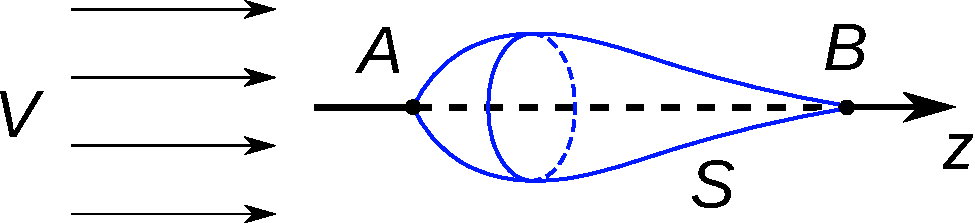
\includegraphics[width=0.8\linewidth]{../img/axisymmetric_body}
}


\frame{
	\frametitle{Продольное обтекание тела вращения}
	\begin{exampleblock}{Метод источников и стоков}
		\parbox{\textwidth}{
			Рассмотрим на оси $Oz$ распределенные источники и стоки с плотностью распределения $\mu(\zeta)$, где $\zeta$ -- положении на оси $Oz$ между точками $A$ и $B$.
		}
	\end{exampleblock}
	
	
	\begin{exampleblock}{Функция тока от источников, распределённых вдоль оси $Oz$ }
		\parbox{\textwidth}{
			\[
			\psi_1(r,z) = -\frac{1}{4\pi}\int\limits_A^B
			\mu(\zeta) \left(
			1 - \frac{z-\zeta}{\sqrt{r^2+(z-\zeta)^2}}
			\right) d\zeta
			\]
		}
	\end{exampleblock}

	\begin{exampleblock}{Функция тока от поступательного потока}
		\parbox{\textwidth}{
			\[
			\psi_2 = -r^2\frac{V}{2}
			\]
			
		}
	\end{exampleblock}
}

\frame{
	\frametitle{Продольное обтекание тела вращения }
	
	\begin{exampleblock}{Искомая функция тока для задачи}
		\parbox{\textwidth}{
			\[
			\psi = \psi_1+\psi_2 = -r^2\frac{V}{2} -\frac{1}{4\pi}\int_A^B
			\mu(\zeta) \left(
			1 - \frac{z-\zeta}{\sqrt{r^2+(z-\zeta)^2}}
			\right) d\zeta
			\]
		}
	\end{exampleblock}\pause

	\begin{exampleblock}{Условие <<непроницаемости>> тела}
		\parbox{\textwidth}{
			\[
			\int_A^B \mu(\zeta) = 0
			\]
			
		}
	\end{exampleblock}\pause

	\begin{exampleblock}{Поверхность тела -- поверхность тока}
		\parbox{\textwidth}{
			\[
			\psi|_S = 0 \quad\Rightarrow\quad
			\frac{1}{4\pi}\int_A^B  \frac{(z-\zeta)\mu(\zeta) d\zeta}{\sqrt{\tilde{r}(z)^2+(z-\zeta)^2}} = 
			\frac{1}{2}V\tilde{r}(z),
			\]
			где $r=\tilde{r}(z)$ -- уравнение дуги $AB$, где $z$ -- координата между точками $A$ и $B$.
		}
	\end{exampleblock}
	
}

\frame{
	\frametitle{Поперечное обтекание тела вращения }
	
	\begin{columns}
		\begin{column}{0.4\textwidth}

			
			\medskip
			\centering
			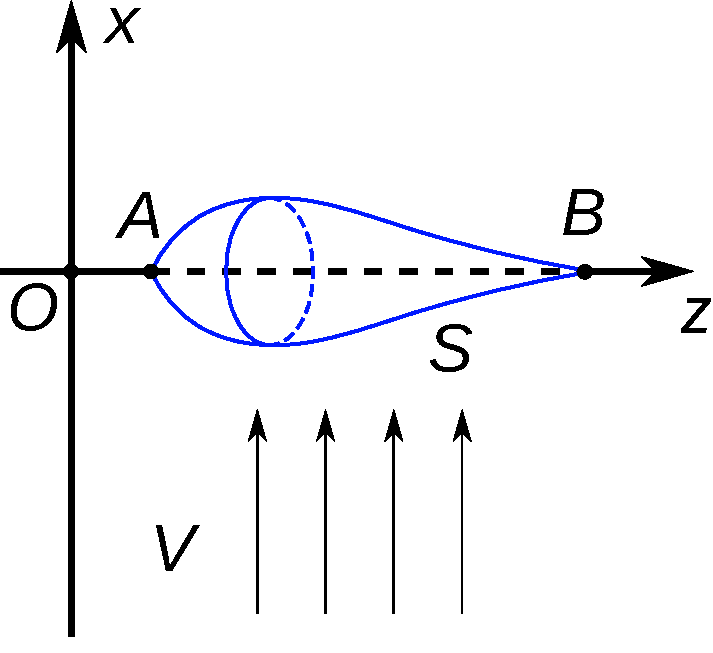
\includegraphics[width=\linewidth]{../img/axisymmetric_body_across}
		\end{column}
		\begin{column}{0.6\textwidth}
		\begin{exampleblock}{Постановка задачи}
			\parbox{\textwidth}{
				
				\medskip
				Требуется найти потенциал или функцию тока течения, описывающие течение идеальной жидкости на бесконечности направленной вдоль оси $Ox$ около тела, образованного вращением заданной дуги $AB$ вокруг оси $Oz$.
			}
		\end{exampleblock}
		\end{column}
	\end{columns}
}


\frame{
	\frametitle{Поперечное обтекание тела вращения }
	
	\begin{exampleblock}{Метод источников и стоков}
	\parbox{\textwidth}{
		Рассмотрим  диполи, распределенные на оси $Oz$, с плотностью распределения $\mu(\zeta)$, где $\zeta$ -- положении на оси $Oz$ между точками $A$ и $B$.
	}
	\end{exampleblock}\pause

	\begin{exampleblock}{Потенциал диполей}
		\parbox{\textwidth}{
		\[
			\varphi_1 = 
			\frac{1}{4\pi}\int\limits_A^B \frac{-\mu(\zeta)x d\zeta}{\left(\sqrt{x^2+y^2+(z-\zeta)^2}\right)^3}=
			\frac{r\cos\theta}{4\pi}
			\int\limits_A^B \frac{-\mu(\zeta) d\zeta}{\left(\sqrt{r^2+(z-\zeta)^2}\right)^3}.
		\]
		}
	\end{exampleblock}
	
	\begin{exampleblock}{Потенциал поступательного движения}
		\parbox{\textwidth}{
		\[
		\varphi_2  = V x = V r \cos\theta
		\]
			
		}
	\end{exampleblock}	
}

\frame{
	\frametitle{Поперечное обтекание тела вращения }
	
	\begin{exampleblock}{Искомый потенциал течения}
		\parbox{\textwidth}{
		\[
			\varphi = \varphi_1 +\varphi_2 = 
			V r \cos\theta - \frac{r\cos\theta}{4\pi}
			\int\limits_A^B \frac{\mu(\zeta) d\zeta}{\left(\sqrt{r^2+(z-\zeta)^2}\right)^3}.
		\]	
		}
	\end{exampleblock}\pause

	\begin{exampleblock}{Уравнения линий тока в цилиндрической системе координат}
		\parbox{\textwidth}{
		\[
			\frac{dr}{v_r} = \frac{dz}{v_z} = \frac{r d\theta}{v_\theta},
			\]
			где
	\only<2>{
			\[
			v_r = \pd{\varphi}{r} = V\cos\theta - \frac{\cos\theta}{4\pi}\pd{}{r} \left\{
			r \int_A^B \frac{\mu(\zeta) d\zeta}{\left(\sqrt{r^2+(z-\zeta)^2}\right)^3}
			\right\},
			\]
	}
	\only<3>{
		\[
		v_z = \pd{\varphi}{z} =
		- \frac{r\cos\theta}{4\pi} \pd{}{z}\left\{
		\int\limits_A^B \frac{\mu(\zeta) d\zeta}{\left(\sqrt{r^2+(z-\zeta)^2}\right)^3}
		\right\},
		\]
	}
	\only<4>{
		\[
		v_\theta = \frac{1}{r}\pd{\varphi}{\theta} =
		-V\sin\theta+
		- \frac{\sin\theta}{4\pi}
		\int\limits_A^B \frac{\mu(\zeta) d\zeta}{\left(\sqrt{r^2+(z-\zeta)^2}\right)^3}.
		\]
	}
			
	}
	\end{exampleblock}	
}

\frame{
	\frametitle{Поперечное обтекание тела вращения }
	
	\begin{exampleblock}{Линии тока на теле вращения}
		\parbox{\textwidth}{
			Линии тока должны проходить вдоль поверхности тела вращения, поэтому соотношение
			\[
			\od{r}{z} =  \frac{v_r}{v_z} = f(r,z) = 
			\frac{
				V - \displaystyle\frac{1}{4\pi}\pd{}{r} \left[
				r \int\limits_A^B \frac{\mu(\zeta) d\zeta}{\left(\sqrt{r^2+(z-\zeta)^2}\right)^3}
				\right]
			}
			{
				- \displaystyle\frac{r}{4\pi} \pd{}{z}\left[
				\int\limits_A^B \frac{\mu(\zeta) d\zeta}{\left(\sqrt{r^2+(z-\zeta)^2}\right)^3}
				\right]
			},
			\]
			где $r=\Phi(z)$ и $\displaystyle\od{r}{z} = \Phi'(z)$ -- заданные функции, описывающие поверхность тела вращения, позволяет найти распределение диполей $\mu(\zeta)$, где $\zeta$ -- координата между точками $A$ и $B$.
		}
	\end{exampleblock}
	
}

\frame{
	\frametitle{ Общий случай обтекания тела вращения }
	
	\begin{exampleblock}{Постановка задачи}
		\parbox{\textwidth}{
			Требуется найти потенциал течения при обтекании тела вращения с поверхностью $S$ поступательным потоком идеальной жидкости со скоростью $\vec{V}$ на бесконечности. 
		}
	\end{exampleblock}


	\centering
	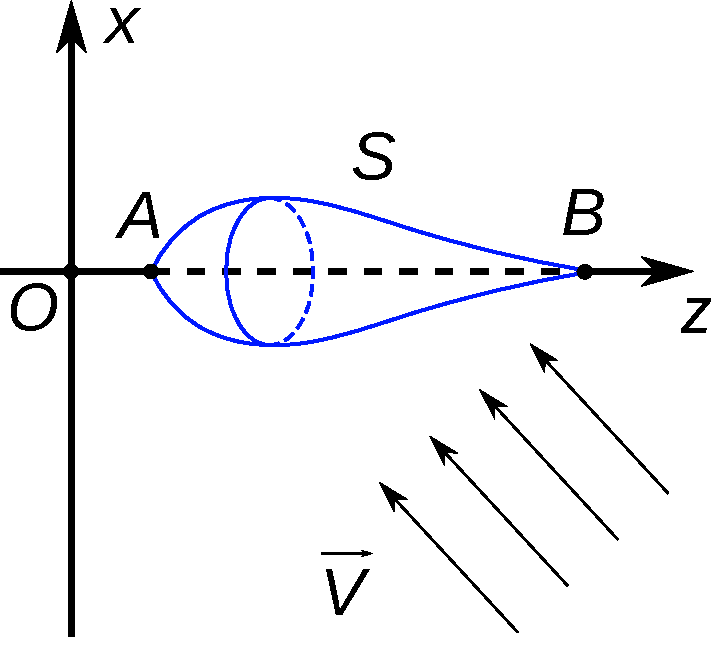
\includegraphics[width=0.5\linewidth]{../img/axisymmetric_body_jeneral}
	
}

\frame{
	\frametitle{ Общий случай обтекания тела вращения }

	\begin{exampleblock}{Математическая постановка задачи}
		\parbox{\textwidth}{
			Всегда можно выбрать систему координат так, чтобы вектор $\vec{V}$ лежал в плоскости $Oxz$, тогда для потенциала течения требуется решить
			\[
			\Delta\varphi = 0
			\]
			при условии на поверхности тела
			\[
			\left. \pd{\varphi}{n} \right|_S = 0
			\]
			и на бесконечности
			\[
			\pd{\varphi}{x} = V_x,\quad
			\pd{\varphi}{y} = 0,\quad
			\pd{\varphi}{z} = V_z.
			\]
		}

	\end{exampleblock}
		
}

\frame{
	\frametitle{Общий случай обтекания тела вращения }
	
	\begin{exampleblock}{Задача обтекания тела продольным потоком со скоростью $V_z$}
		\parbox{\textwidth}{
		\[
		\Delta\varphi_1 = 0,\quad
		\left. \pd{\varphi_1}{n} \right|_S = 0,\quad
		\pd{\varphi_1}{x} = \alert{0},\quad
		\pd{\varphi_1}{y} = 0,\quad
		\pd{\varphi_1}{z} = \alert{V_z}.
		\]
		}
	\end{exampleblock} \pause


	\begin{exampleblock}{Задача обтекания тела поперечным потоком со скоростью $V_x$}
		\parbox{\textwidth}{
		\[
			\Delta\varphi_2 = 0,\quad
			\left. \pd{\varphi_2}{n} \right|_S = 0,\quad
			\pd{\varphi_2}{x} = \alert{V_x},\quad
			\pd{\varphi_2}{y} = 0,\quad
			\pd{\varphi_2}{z} = \alert{0}.
		\]
			
		}
	\end{exampleblock}\pause

	\begin{exampleblock}{Искомый потенциал}
		\parbox{\textwidth}{
			\[
			\varphi = \varphi_1 + \varphi_2.
			\]
		}
	\end{exampleblock}
}

\frame{
	\frametitle{ Литература }
	\begin{itemize}[partopsep=1pt,label=\textbullet]
		\item 
		{\em Кочин~Н.~Е., Кибель~И.~А., Розе~Н.~В.} Теоретическая гидромеханика. М.:Гос. издат. физ.-мат. лит., 1963.
		\item {\em Валландер~С.~В.} Лекции по аэрогидромеханике. Учеб. пособие. Л., Изд-во Ленингр. ун-та, 1978. 
	\end{itemize}
}
 
\end{document}